\chapter{Motion planning theory}\label{cha:motion_planning}
\section{General definitions and terminology}
Motion planning is defined as the task of finding a
path from a starting state to a goal state which fulfills a given set of constraints, while minimizing some 
performance measure.
These constraints might include differential constraints of the system and obstacle avoidance among others.
Common performance measures include minimal time or minimal energy required.
We begin with introducing general definitions and terminology that are used to
describe motion planning in this thesis. A broad reference covering the multiple aspects of motion planning is given in 
\cite{planning_algorithms}.
\subsection{Graph terminology}
We first introduce the mathematical concept of graphs, following the definitions in \cite{graph_theory}.

\begin{definition}[Graph]
    A \textit{graph} is defined as a set $\mathcal{G}=\langle\mathcal{V},\mathcal{E}\rangle$ 
    where $\mathcal{V}$ are the \textit{vertices} of the graph and $\mathcal{E}$ are the \textit{edges}.
    Two vertices $v_i,v_j\in\mathcal{V}$ might be connected by an edge $e_{i,j}\in\mathcal{E}$ or not connected.
\end{definition}
    
\begin{definition}[Weighted graph]
    In a \textit{weighted graph}, each edge is assigned a cost $C(e)\in\mathrm{R}$. 
\end{definition}


\begin{definition}[Directed graph]
    In a \textit{directed} graph, it is possible that $c_{i,j}\neq c_{j,i}$ and
    there might not be an edge $e_{j,i}$ even if $e_{i,j}\in\mathcal{E}$.
\end{definition}

\begin{definition}[Path]
    A \textit{path} in a weighted and possibly directed graph is defined as a set of edges
    $\mathcal{V}_p\subset\mathcal{V}$ and edges $\mathcal{E}_p\subset\mathcal{E}$ where the vertices in 
    $\mathcal{V}_p$ are connected by the edges in $\mathcal{E}_p$, and each edge and vertex occurs only once.
    The total \textit{cost} of a path is defined as
    \begin{equation}
        C(\mathcal{V}_p, \mathcal{E}_p)=\sum_{e\in\mathcal{E}_p}C(e)
    \end{equation}
\end{definition}

\subsection{Motion planning terminology}
We further define some common terms used in motion planning.

\begin{definition}[State and action spaces]
    We define the \textit{state space} $\mathcal{X}$ and \textit{action space}
    $\mathcal{U}$ as the set of obtainable states $x$ and available actions $u$ for the
    studied system.
    $\mathcal{X}$ can be further divided into
    \begin{equation}
        \mathcal{X} = \mathcal{X}_{free} + \mathcal{X}_{obs}
    \end{equation}
    where $\mathcal{X}_{obs}$ are states which contain some kind of obstacle. 
\end{definition}

\begin{definition}[Motion plan]
    A motion plan is defined as a sequence of states
    \begin{equation}
        \{x(t_1),\hdots, x(t_n)\}\in\mathcal{X}_{free}
    \end{equation}
    and actions
    \begin{equation}
        \{u(t_1),\hdots,u(t_n)\}\in\mathcal{U}
    \end{equation}
    which takes the system from a specified initial state $x(t_1)=x_i$ to a 
    goal state $x(t_n)=x_f$ while fulfilling
    \begin{equation}
        x(t_{i+1})=x(t_i) + \int_{t_i}^{t_{i+1}} f(x, u) dt
    \end{equation}
    where $f(x, u)$ is called the \textit{transition function} \cite{planning_algorithms}.
\end{definition}

\subsection{Differential constraints}
Differential constraints restrict the set of possible actions and states that 
the system can obtain. An important class of systems under differential constraints 
are \textit{non-holonomic} systems.

\begin{definition}[Non-holonomic system]
    In a \textit{non-holonomic} system, the current state $x(t)$ is dependent 
    on in which order the actions $u(t_i),\quad t_i<t$ where performed.
\end{definition}

A formal definition and extensive discussion of non-holonomic systems is given 
in \cite[Chapter~15]{planning_algorithms}. Systems only capable of motion in a direction 
dependent on the current state, such as cars and fixed-wing UAVs belong to this class of systems.

\section{Sampling based motion planning}
Both $\mathcal{X}$ and $\mathcal{U}$ are generally continuous, and need to be sampled 
in some way. This means that the resulting path will only be \textit{resolution complete}, i. e. 
the optimality of the plan will depend on the sampling resolution $d$. In sampling based
motion planning a \textit{reachability graph} is commonly used \cite{planning_algorithms}.

\begin{definition}[Reachability graph]\label{def:reach_graph}
    Given a starting state $x_0(t_0)\in\mathcal{X}_d$, we define the \textit{reachable set} 
    $R(x_0, \mathcal{U}_d)$ as the set of states which are reached by applying any action $u\in\mathcal{U}_d$.
    By incrementally calculating the reachable set for each $x\in R(x_0, \mathcal{U}_d)$ we create the \textit{reachability tree} $\mathcal{T}_r(x_0, \mathcal{U}_d)$.
    The reachability tree is a directed graph where each vertex consists of a state $x$ which is reachable from $x_0$ by applying some action sequence 
    $\{u_1,\hdots,u_n\}\in\mathcal{U}_d$. By pruning any duplicate states from $\mathcal{T}_r$ we finally reach the \textit{reachability graph} $\mathcal{G}_r(x_0, \mathcal{U}_d)$
\end{definition}

\subsection{Forward simulation}
The next state in $G_r$ given a specified input action $u$ is obtained by 
integrating the transition function $f(x, u)$ on $[0, \Delta t]$. In practice this 
integral is calculated using some numerical approximation method. A common choice is the 
fourth-order \textit{Runge-Kutta integration method}, which is defined in \cite{planning_algorithms} as
\begin{equation}
    x(\Delta t)\approx x(0) + \frac{\Delta t}{6}(w_1 + 2w_2 + 2w_3 + w_4)
\end{equation}
where
\begin{align}
\begin{split}
    w_1 &= f(x(0), u) \\
    w_2 &= f(x(0) + \frac{1}{2}\Delta t w_1, u) \\
    w_3 &= f(x(0) + \frac{1}{2}\Delta t w_2, u) \\
    w_3 &= f(x(0) + \Delta t w_3, u)
\end{split}
\end{align}

\subsection{Motion primitives}\label{sec:motion_prim}
Often it is not feasible nor desirable to sample from all possible actions in $\mathcal{U}_d$.
A common method is to instead create a set of \textit{motion primitives} $\mathcal{P}$ which consists of 
sequences of actions that take the system from desired initial and final states \cite{state_lattice_planning}.

\textit{Maneuver-based} motion primitive generation is introduced in \cite{Bergman_lic} as
the method of generating $\mathcal{P}$ based on a fixed set of maneuvers. One such 
maneuver is \textit{heading change}, which is defined as taking the system from an initial heading $\psi_i$ to a final heading $\psi_f$.
This primitive set can be generated by solving the optimal control problem
\begin{subequations}
    \label{eq:opt_problem_mp}
    \begin{alignat}{3}
    &\min_{x(t),u(t),T}        &\qquad& J=\Phi(x(T),T) + \int_{0}^{T} l(x(t),u(t))dt & \\
    &\text{subject to} & & \psi(0)=0,\quad \psi(T)=\Delta\psi &\\
    & & & \dot{x}=f(x(t), u(t)) &t\in[0,T]\\
    & & & x(t)\in\mathcal{X}& t\in[0,T]\\
    & & & u(t)\in\mathcal{U} & t\in[0,T]
    \end{alignat}
\end{subequations}
Where $\Delta\psi=\psi_f-\psi_i$ and the performance metrics $\Phi(x(T), T)$ and $l(x(t),u(t))$ are chosen such that a desired property, such as 
required energy or time is minimized. The motion primitive set $\mathcal{P}$ then consists of the 
solutions of \eqref{eq:opt_problem_mp} for different values of $\Delta\psi$.
\section{Graph search methods}
The problem of finding the minimum cost path between two vertices in a graph $\mathcal{G}$
is well studied, and there are numerous algorithms for solving it. These algorithms regularly require that 
$C(e)\geq0 \forall e\in\mathcal{E}$. By using such algorithms together with the concept of 
reachability graphs defined in \eqref{def:reach_graph} resolution-optimal motion plans can be calculated \cite{Bergman_lic}. 

\subsection{A-star search}\label{sec:a-star}
The $A^*$ algorithm was introduced in \cite{astar} and is widely used to find the shortest path in graphs.
Two important components of this algorithm is the \textit{cost-to-come} $g(x)$ and \textit{heuristic} $h(x)$. $g(x)$ is defined as 
the cost of the shortest path from the starting state $x_i$ to $x$, and $h(x, x_f)$ as the cost of the shortest path from $x$ to the goal $x_f$.
Thus for any state $x$ the total cost for a path through this state to the goal is given as $g(x)+h(x,x_f)$.
Often the true value of $h(x, x_f)$ is not known and has to be approximated by some other function $h'(x, x_f)$. A necessary 
condition for optimality of the resulting path is that $h'(x, x_f)$ is \textit{admissible}, as defined below.

\begin{definition}[Admissible heuristic]
    A heuristic function $h'(x, x')$ is \textit{admissible} if
    \begin{equation}
        h'(x, x')\leq h(x, x') \quad\forall x
    \end{equation}
    where $h(x, x_f)$ is the true heuristic value.    
\end{definition}

An outline of motion planning with $A^*$ is presented in Algorithm \ref{alg:astar}.
The function $\text{EXPAND}(x, \mathcal{P})$ returns all states reached from $x$ by applying motion primitives in $\mathcal{P}$ and the associated cost of each primitive. The function $\text{POP}(\mathcal{O})$ returns the state in
the open set with the lowest estimated total cost, 
and \\$\text{CURRENT\_COST}(x,\mathcal{O})$  returns the estimated cost currently stored for $x$. 


\begin{algorithm}
    \begin{algorithmic}
        \Require Motion primitive set $\mathcal{P}$, valid states $\mathcal{X}_{free}$, initial state $x_i$, final state $x_f$, open set $\mathcal{O}$, closed set $\mathcal{C}$
            \State $\mathcal{C}\gets \{x_i\}$
            \State $\mathcal{O}\gets\text{EXPAND}(x_s, \mathcal{P})$
            \While{$\mathcal{O}\neq \emptyset$}
                \State $(x,g(x))\gets \text{POP}(\mathcal{O})$
                \If{$x==x_{f}$} \Comment{Goal found}
                    \State \textbf{return} $g(x)$
                \EndIf
                \ForAll{$(x',c')\in\text{EXPAND}(x,\mathcal{P})$}
                    \If{$x'\in\mathcal{X}_{free}$ \textbf{and} $x'\notin \mathcal{C}$}
                        \State $c_{tot}=g(x) + c' + h'(x', x_{g})$ \Comment Estimate total cost
                        \State $c\gets\text{CURRENT\_COST}(x', \mathcal{O})$
                        \If{$x'\notin \mathcal{O}$ \textbf{or} $c > c_{tot}$}
                            \State $\mathcal{O}\gets\mathcal{O}\bigcup\{(x',c_{tot})\}$\Comment Update total cost estimate
                        \EndIf
                    \EndIf
                \EndFor
            \State $\mathcal{C}\gets\mathcal{C}\bigcup \{x\}$
            \EndWhile
        \end{algorithmic}
        \caption{$A^*$ based motion planning}
        \label{alg:astar}
\end{algorithm}

\subsection{Hybrid A-star}
A disadvantage of the original $A^*$ formulation in motion planning is that it only allows the states to take on discrete values $x_d$. This was extended in \cite{hybrid_astar} to the Hybrid $A^*$ formulation,
which allows continuous states. To discretize the state-space it is divided into cells, and states in the same cell are considered equal. The difference from the classic $A^*$ formulation is illustrated in 
Figure \ref{fig:hybrid_vs_regular}.

\begin{figure}
    \begin{center}
        \tikzstyle{dot}=[
            circle,
            fill=black,
            inner sep=0pt,
            minimum width=5pt
        ]
        \subfloat[Regular $A^*$]{
            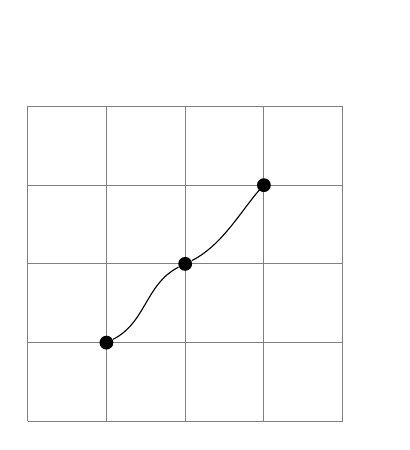
\begin{tikzpicture}
                \useasboundingbox (0, 0) rectangle (4.5, 5);
                \draw[gray] (0,0) grid (4,4);
                \node[dot](start) at (1,1){};
                \node[dot](end) at (2,2){};
                \node[dot] at (3,3){};
    
                \draw (start) .. controls (1.5,1.25) and (1.5,1.75) .. (end);
                \draw (end) .. controls (2.5,2.25) and (2.75,2.75) .. (3,3);
            \end{tikzpicture}
        }
        \subfloat[Hybrid $A^*$]{
            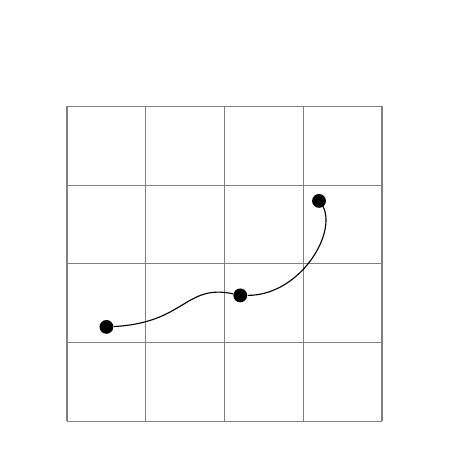
\begin{tikzpicture}
                \useasboundingbox (-0.5, 0) rectangle (4.5, 5);
                \draw[gray] (0,0) grid (4,4);
                \node[dot](start) at (0.5,1.2){};
                \node[dot](end) at (2.2,1.6){};
                \node[dot] at (3.2,2.8){};
                \draw (start) .. controls (1.5,1.25) and (1.5,1.75) .. (end);
                \draw (end) .. controls (3,1.6) and (3.5,2.5) .. (3.2,2.8);
            \end{tikzpicture}
        }
    \end{center}
    \caption{Difference between regular and hybrid $A^*$}
    \label{fig:hybrid_vs_regular}
\end{figure}

The Hybrid $A^*$ algorithm also includes the concept of \textit{analytic expansions}, which means that the
model of the current system is simulated from the current state $x$ to the goal $x_f$. If this simulated path is feasible,
i. e. doesn't collide with obstacles the algorithm returns. It was shown that this inclusion improved execution speed of the algorithm,
and it also allows the goal state to be exactly reached instead of the closest discrete state.

\subsection{Non-holonomic heuristics}
A common choice of heuristic function is simply the euclidean distance $h'(x, x_f)=\|x_f-x\|$. However, in many cases for
non-holonomic systems this measure greatly underestimates the actual cost-to-go, which leads to unnecessary node expansions and 
increased computation time of the algorithm. It is therefore desirable to use another heuristic which takes the non-holonomic properties 
of the system into account \cite{state_lattice_planning}.
\subsubsection{Dubin's metric}
Dubin's path was introduced in \cite{dubins} and provides an analytical solution for the
shortest path between two points $(x_i,y_i,\psi_i)$ and $(x_f,y_f,\psi_f)$ with a constraint on maximal turn-rate $|\dot{\psi}|\leq\dot{\psi}_{max}$.
The length of a Dubin's path between $x$ and $x'$ has been widely used as a heuristic for non-holonomic systems only capable of forward motion, such as car-like robots and fixed-wing UAVs \cite{2_phase_uav}.
\subsubsection{Heuristic Look-Up Table}\label{sec:hlut}
Another efficient method for non-holonomic systems is to pre-compute the optimal cost from a number of start states to 
a large number of goal states and store these in a Heuristic Look-Up Table (HLUT) \cite{hlut}. However, since the HLUT 
must be finite in size, some fallback heuristic such as euclidean distance has to be used if the value of $h(x,x')$ is not available for some $x$ and $x'$.
This means that some trade-off between HLUT size and algorithm efficiency has to be made, and states where the difference between $h(x,x')$ and the fallback heuristic 
should be prioritized for inclusion. Given a set of motion primitives $\mathcal{P}$ the HLUT can be efficiently generated using Dijkstra's algorithm. 
An outline of this method is given in Algorithm \ref{alg:hlut}, where $\mathcal{X}$ is the set of states for which we want to generate HLUT values, and the function definitions 
are equal to the ones in Algorithm \ref{alg:astar}.

\begin{algorithm}
    \begin{algorithmic}
        \Require Motion primitive set $\mathcal{P}$, valid states $\mathcal{X}$, initial state $x_i$, open set $\mathcal{O}$, closed set $\mathcal{C}$
            \State $\mathcal{C}\gets \{x_i\}$
            \State $\mathcal{O}\gets\text{EXPAND}(x_i, \mathcal{P})$
            \While{$\mathcal{O}\neq \emptyset$}
                \State $(x,g(x))\gets \text{POP}(\mathcal{O})$
                \ForAll{$(x',c')\in\text{EXPAND}(x,\mathcal{P})$}
                    \If{$x'\in\mathcal{X}$ \textbf{and} $x'\notin \mathcal{C}$}
                        \State $c_{tot}=g(x) + c'$ \Comment Calculate cost-to-go
                        \State $c\gets\text{CURRENT\_COST}(x', \mathcal{O})$
                        \If{$x'\notin \mathcal{O}$ \textbf{or} $c > c_{tot}$}
                            \State $\mathcal{O}\gets\mathcal{O}\bigcup\{(x',c_{tot})\}$\Comment Update cost-to-go
                        \EndIf
                    \EndIf
                \EndFor
            \State $\mathcal{C}\gets\mathcal{C}\bigcup \{x\}$
            \State $\text{HLUT}(x_i,x)=g(x)$\Comment Store value in HLUT
            \EndWhile
        \end{algorithmic}
        \caption{HLUT generation using Dijkstra's algorithm}
        \label{alg:hlut}
\end{algorithm}

\subsection{Inflated heuristics and sub-optimality guarantees}\label{sec:sub_optimal}
If $h'(x, x')$ is an admissible heuristic and we instead use the heuristic $\epsilon h'(x, x')$ for some $\epsilon>1$ during planning,
the resulting path is not guaranteed to be optimal. However, an important result is that the sub-optimal path is guaranteed to be at most $\epsilon$ times 
longer than the optimal one. This property is exploited in so-called anytime algorithms, since inflating the heuristic value often leads to much faster solutions which is 
desirable in realtime implementations \cite{anytime_astar}. 